\documentclass{ucalgthes1}   
\usepackage[letterpaper,top=1in, bottom=1.22in, left=1.40in, right=0.850in]{geometry}
\usepackage{fancyhdr}
\fancyhead{}
\fancyfoot{}
\renewcommand{\headrulewidth}{0pt}
\fancyhead[RO,LE]{\thepage}  
\usepackage{hyperref}

\usepackage{algorithm}
\usepackage{algorithmic}
\usepackage{amsfonts}
\usepackage{amsmath}
\usepackage{amssymb}
\usepackage{amsthm}
\usepackage{comment}
\usepackage{float}
\usepackage{graphics}

\theoremstyle{plain}
\newtheorem{thm}{Theorem}[section]
\newtheorem{lemma}[thm]{Lemma}
\newtheorem{prop}[thm]{Proposition}
\newtheorem{cor}[thm]{Corollary}
\theoremstyle{definition}
\newtheorem{defn}[thm]{Definition}

\renewcommand{\algorithmicrequire}{\textbf{Input:}}
\renewcommand{\algorithmicensure}{\textbf{Output:}}

\newcommand{\CC}{\mathbb{C}}
\newcommand{\NN}{\mathbb{N}}
\newcommand{\RR}{\mathbb{R}}
\newcommand{\KK}{\mathbb{K}}
\newcommand{\MM}{\mathcal{M}}
\newcommand{\OO}{\mathcal{O}}
\newcommand{\ZZ}{\mathbb{Z}}
\newcommand{\QQ}{\mathbb{Q}}
\newcommand{\NP}{\textrm{NP}}
\newcommand{\RRgtz}{\mathbb{R}_{>0}}
\newcommand{\ZZgtz}{\mathbb{Z}_{>0}}
\newcommand{\ZZgez}{\mathbb{Z}_{\ge 0}}
\newcommand{\QQgtz}{\mathbb{Q}_{>0}}
\newcommand{\QQgez}{\mathbb{Q}_{\ge 0}}
\newcommand{\matrixto}[2]{\left( \begin{array}{rr} #1 & #2 \end{array} \right)}
\newcommand{\matrixot}[2]{\left( \begin{array}{r} #1 \\ #2 \end{array} \right)}
\newcommand{\matrixtt}[4]{\left( \begin{array}{rr} #1 & #2 \\ #3 & #4 \end{array} \right)}
\newcommand{\ntoinfty}{\lim_{n \rightarrow \infty}}
\newcommand{\floor}[1]{\left\lfloor #1 \right\rfloor}
\newcommand{\ceil}[1]{\left\lceil #1 \right\rceil}

\begin{document}

\setcounter{chapter}{2}
\chapter{Exponentiation}

Given a group $G$, an element $g \in G$, and an integer $n$, computing $g^n$ is a common operation and is known as exponentiation.  Diffie-Hellman key exchange is an example that uses exponentiation whereby two parties can jointly establish a shared secret key over an insecure channel.  Another application discussed in more detail in this thesis is that of computing the order of a group element.  Our approach, in this case, is to exponentiate a group element to the product, $P$, of several small prime powers.  The result is an element whose order is likely to not by divisible by any of these primes. The order of this new element is then computed using a variant of Shanks' baby-step giant-step algorithm where only powers relatively prime to $P$ need to be computed.  Determining the order of an element can be useful in computing the structure of a group, or in factoring an integer associated with a group.  In these examples, being able to exponentiate faster means that the complete program can run more quickly.

In Sections \ref{section:binary} and \ref{section:naf} we discuss standard exponentiation techniques that rely on a base 2 representation of the exponent.  The method using non-adjacent form described in Section \ref{section:naf} also benefits when the cost of computing the inverse of a group element is inexpensive or relatively free.  In Section \ref{section:dbns} we introduce double-base number systems, which, as the name implies, are number systems that make use of multiple bases in the representation of a number. In Section \ref{section:dbnsMethods} we discuss some methods to compute double-base representations found in the literature.  In this thesis, we pay particular attention to double-base representations that use bases 2 and 3, since a representation using base 3 can benefit when the cost of cubing an element is less than the cost of multiplying an element with its square.


%%%%%%%%%%%%%%%%%%%%%%%%%
% BINARY EXPONENTIATION %
%%%%%%%%%%%%%%%%%%%%%%%%%
\bigbreak
\section{Binary Exponentiation}\label{section:binary}
Perhaps the simplest method of exponentiation is that of binary exponentation.  Let $g$ be an element in the group $G$ and $n$ be an integer.  We want to compute $g^n \in G$.  We first represent $n$ in binary as
\[
	n = \sum_{i=0}^{\floor{log_2 n}} b_i 2^i
\]
where $b_i \in \{0, 1\}$ such that $b_i$ represents the $i^{\textrm{th}}$ bit of $n$.   We compute $g^{2^i}$ by repeated squaring of $g$ and compute $g^n$ by computing
\[
	g^n = \prod_{i=0}^{\floor{log_2 n}} g^{b_i 2^i}.
\]
This description is known as right-to-left binary exponentiation as the result is computed by evaluating the bits of the exponent $n$ from low order to high order.  The left-to-right variant evaluates the bits of the exponent $n$ from high order to lower order by repeatedly squaring the result and multiplying this with the base element $g$ when $b_i = 1$.  The left-to-right variant has the advantage that one of the values in the multiplication, namely $g$, remains constant throughout the evaluation.  There also exist windowed variants where $g^w$ is precomputed for each $w$ in some window $0 \le w \le 2^k$ for some $k$ (typically chosen to be cache efficient). The exponent $n$ is then expressed in base $2^k$.  There are numerous sources discussing windowed variants such as (TODO) but, we do not discuss these variants further here.

Binary exponentiation algorithms require $\floor{log_2 n}$ squarings and on average $\floor{log_2 n}/2$ multiplications, since a multiplication is only necessary when $b_i = 1$ and the probability of $b_i = 1$ is 1/2.

%%%%%%%%%%%%%%%%%%%%%%
% NAF EXPONENTIATION %
%%%%%%%%%%%%%%%%%%%%%%
\bigbreak
\section{Non-Adjacent Form Exponentiation}\label{section:naf}

The Non-Adjacent Form (NAF) of an integer is a \emph{signed} base two representation such that no two non-zero terms in the representation are adjacent. This last requirement ensures that there is only one representation for a given integer $n$. Formally, an integer $n$ is represented such that
\[
	n = \sum_{i=0}^{\floor{log_2 n}+1} s_i 2^i
\]
where $s_i \in \{0, 1, -1\}$ and $s_i \cdot s_{i+1} = 0$. For example, suppose $n = 23814216$.  In binary we have
\begin{equation}\label{eq:binaryEg}
	23814216 = 2^3+2^6+2^{13}+2^{14}+2^{16}+2^{17}+2^{19}+2^{21}+2^{22}+2^{24}
\end{equation}
and in non-adjacent form we have
\begin{equation}\label{eq:nafEg}
	23814216 = 2^3+2^6-2^{13}-2^{15}-2^{18}-2^{20}-2^{23}+2^{25}.
\end{equation}
Similar to the binary case, we can compute $g^n$ using
\[
	g^n = \prod _{i=0}^{\floor{log_2 n}+1} g^{s_i 2^i}.
\]
Since $s_i$ can be $-1$ and inversion can be expensive, we can instead compute the product as
\[
	g^n = \left( \prod_{i : s_i=1} g^{2^i} \right) \cdot \left( \prod_{i : s_i=-1} g^{2^i} \right)^{-1}
\]
which requires at most one inversion.

A typical method to compute the non-adjacent form of an integer $n$ is to inspect $n$ two bits at a time from least significant to most significant.  Let $n=\sum b_i2^i$ be the binary representation of $n$ and let $j=0$.  If the bit pattern $\langle b_{j+1}, b_j \rangle = 01$, then let $s_j = 1$ and subtract $2^j$ from $n$.  If $\langle b_{j+1}, b_j \rangle = 11$, then let $s_j = -1$ and add $2^j$ to $n$.  When the bit pattern $\langle b_{j+1}, b_j \rangle$ is $00$ or $10$, let $s_j = 0$. Next, increment $j$ and repeat while $n \ne 0$.

In our experiments, we use a variation of the above, given in \cite[p.4]{Joye2000}, that maintains a carry flag $c$.  Instead of adding $2^i$ to $n$, we set $c = 1$, and instead of subtracting $2^i$ from $n$, we set $c = 0$.  When inspecting $n$ two bits at a time, we consider the bit pattern $(m+c) \bmod 4$ where $m = 2 b_{i+1} + b_i$.  For large enough $n$, the cost of addition and subtraction is reduced from $O(\log n)$ to $O(1)$.  This technique is given in Algorithm \ref{alg:nafR2LImmutable}.

A particular advantage of a non-adjacent form exponentiation over a binary exponentiation is the number of operations required.  While the binary method requires $\floor{\log_2 n}$ squares and on average $\floor{\log_2 n}/2$ multiplications, a non-adjacent form exponentiation requires at most $\floor{\log_2 n}+1$ squares and on average $(\floor{\log_2 n}+1)/3$ multiplications.  To see this, recall that non-adjacent form requires that no two non-zero terms be adjacent.  Consider any two adjacent terms.  The possible outcomes are $(0,0)$, $(s, 0)$, or $(0, s$) where $s \in \{-1, 1\}$. This means that 2/3 of the time, 1/2 of the terms will be non-zero, and so the probability of any given term being non-zero is 1/3.


%%%%%%%%
% DBNS %
%%%%%%%%
\bigbreak
\section{Double-Base Number Systems}\label{section:dbns}

A significant advantage of non-adjacent form over a binary representation is that on average the number of non-zero terms (the density of the representation) is lower.  This can be even better when we extend the representation to a signed double-base number system (DBNS).  Binary and non-adjacent form are both a base 2 number system.  In the case of a double base number system, as the name suggests, we use two bases.  This system was first introduced by Dimitrov and Cooklev \cite{Dimitrov1995}.  Given two coprime integers $p$ and $q$ and some integer $n$, we represent $n$ as the sum and difference of the product of powers of $p$ and $q$,
\begin{equation}\label{eq:generalDbnsForm}
	n = \sum_{i=1}^k s_i p^{a_i} q^{b_i}
\end{equation}
where $s_i \in \{-1, 1\}$ and $a_i, b_i, k \in \ZZgez$.

Since this thesis focuses on exponentiation in the ideal class group, and since we can compute the square of an element faster than multiplying it with itself, and we can compute the cube of an element faster than multiplying its square with itself, we will be particularly interested in bases $p=2$ and $q=3$.  In other words, we will focus on representations of $n$ such that $n = \sum_{i=1}^k s_i 2^{a_i} 3^{b_i}$.

As an example of a 2,3 double-base representation, consider the number $n=23814216$ again.  Given the bases $p=2$ and $q=3$, \emph{one} possible representation of $n$ is
\begin{equation}\label{eq:unchainedEg}
	23814216 = 2^3 3^3 - 2^4 3^6 - 2^8 3^5 + 2^{15} 3^6.
\end{equation}
Another possible representation is
\begin{equation}\label{eq:chainedEg}
	23814216 = 2^3 3^2 -2^{13} 3^2 +2^{15} 3^6.
\end{equation}
Different representations will trade off cubings for squarings and the best representation will depend on the needs of the application.  Later, we shall see some algorithms that take this into account, but many are designed to either find representations quickly, representations of a special form, or representations with few terms.

Recall, the binary representation \eqref{eq:binaryEg}, non-adjacent form \eqref{eq:nafEg}, and a 2,3 double-base representation \eqref{eq:chainedEg} of 23814216 were
\begin{align*}
	23814216 &= 2^3+2^6+2^{13}+2^{14}+2^{16}+2^{17}+2^{19}+2^{21}+2^{22}+2^{24}, & \mbox{\{using binary\}} \\
	23814216 &= 2^3+2^6-2^{13}-2^{15}-2^{18}-2^{20}-2^{23}+2^{25}, & \mbox{\{using NAF\}} \\
	23814216 &= 2^3 3^2 -2^{13} 3^2 +2^{15} 3^6. & \mbox{\{using 2,3 DBNS\}}
\end{align*}
The binary representation has 10 terms, while the non-adjacent form has only 8 terms.  The 2,3 representation given above contains only three terms.  While a non-adjacent form has in expectation $\floor{\log_2 n}/3$ terms and a binary representation has in expectation $\floor{\log_2 n}/2$ terms, both are bounded by $O(\log n)$ in the number of terms.  Ciet and Sica \cite{Ciet2005} give an algorithm for 2,3 double-base representations, where they prove that the number of terms is bounded by $O(\log n / \log \log n)$.  For this reason, many algorithms focus on reducing the number of terms in a 2,3 representation.   Naturally, the time to compute a 2,3 double-base exponentiation is further reduced if the corresponding cost to compute $g^2$ is less than the cost to compute $g \cdot g$, or the cost to compute $g^3$ is less than the cost to compute $g^2 \cdot g$. 

%%%%%%%%%%%%%%%%%%%%%%%%%%%%%%%%%%%%%%%
\bigbreak
\subsection{Chains vs. Representations}

One way to classify algorithms that compute 2,3 representations is by the constraints placed on the \emph{partition} of an integer $n$.  For an example of a partition, consider the 2,3 representation of $23814216 = 2^3 3^2 -2^{13} 3^2 +2^{15} 3^6$.  The terms $2^3 3^2$, $2^{13} 3^2$, and $2^{15} 3^6$ when monotonically increasing by absolute value is a partition of the integer $23814216$.  

\begin{defn}
A partition of an integer $n = x_1 \pm x_2 \pm \cdots \pm x_k$ is \emph{chained} if every term $x_i$ divides every term $x_j$ for $i < j$ and $x_i \le x_j$. A partition is said to be \emph{strictly chained} if it is chained and $x_i$ is \emph{stricly} less than $x_j$ for each $i < j$.
\end{defn}

\noindent
Binary and non-adjacent form are special types of strictly chained partitions, since for any two non-zero terms $x_i = |s_i2^i|$ and $x_j = |s_j2^j|$ where $i < j$ we have $x_i ~|~ x_j$ and $x_i < x_j$.  The 2,3 representation of $23814216 = 2^3 3^2 - 2^{13} 3^2 + 2^{15} 3^6$ is an example of a chained partition, since $2^3 3^2 ~|~ 2^{13} 3^2 ~|~ 2^{15} 3^6$.

The benefit of restricting 2,3 representations to chained representations is the ease with which one can compute $g^n$ when $n$ is given as a chain.  For example $g^{23814216} = g^{2^3 3^2 - 2^{13} 3^2 + 2^{15} 3^6}$ can be computed by first computing $x_1 = g^{2^3 3^2}$, $x_2 = {x_1}^{2^{10}}$, $x_3 = {x_2}^{2^2 3^4}$, and finally $g^{23814216} = \left(x_1 \cdot x_3\right) \cdot \left(x_2\right)^{-1}$.  Algorithm \ref{alg:expWithChain} can be used to compute $g^n$ for $g \in G$ and $n$ given as a chained 2,3 representation.  The cost of algorithm \ref{alg:expWithChain} is as follows: Let $n$ be defined as $\sum_{i=1}^k s_i p^{a_i}q^{b_i}$, let $max_a = \max \{a_1,...,a_k\}$, and let $max_b = \max \{b_1,...,b_k\}$.  Then we require $max_a$ squares, $max_b$ cubes, $k-1$ multiplications, and at most one inverse.  Since $x_i ~|~ x_{i+1}$, we need only retain $x_i$ in order to compute $x_{i+1}$. For this reason, many algorithms that find 2,3 representations constrain these representations to be chains.


%%%%%%%%%%%%%%%%%%%%%%%%%%%%%%%%%%%%%%%%%%%%%%%%%%%%%%%
\bigbreak
\subsection{Exponentiating general 2,3 representations}

Another class of algorithms compute representations without the constraint that larger terms be divisible by smaller terms.  Given a general 2,3 representation for an integer $n = \sum_{i=1}^k s_i 2^{a_i} 3^{b_i}$, M\'{e}loni and Hasan \cite[Section 3.2]{Meloni2009} use a modification of Yao's Algorithm to achieve the same bound on the number of operations as in algorithm \ref{alg:expWithChain}, but with a bound of $O(\min \{max_a, max_b\})$ on the memory used.  Suppose $max_b < max_a$.  We require the terms to be labelled and sorted such that $a_1 \ge ... \ge a_k$.  The algorithm works by precomputing a table of $T_b = g^{3^b}$ for $0 \le b \le max_b$.  Let $i=1$ and begin with the first term $s_i2^{a_i}3^{b_i}$.  We look up $T_{b_i} = g^{3^{b_i}}$ and, after applying the sign $s_i$, we multiply ${T_{b_i}}^{s_i}$ with the running result.  Let $a_\Delta = a_i - a_{i+1}$ when $i < k$ and $a_\Delta = a_k$ when $i = k$.  It then squares the running result $a_\Delta$ times.  The algorithm removes the term $s_i2^{a_i}3^{b_i}$ from the list of terms, and continues in this way with the term with the next largest $a_i$.  The algorithm terminates when there are no more terms in the list.  Algorithm  \ref{alg:yaos} gives pseudo-code for this approach and requires $O(max_b)$ memory.  When $max_a < max_b$, we use a related algorithm that requires the terms to be sorted such that $b_1 \ge ... \ge b_k$; it precomputes $T_a = g^{2^a}$ for $0 \le a \le max_a$ and works similar to Algorithm \ref{alg:yaos} but with cubing and squaring appropriately swapped.

For example, the 2,3 representation $23814216 = 2^{15} 3^6 - 2^8 3^5 - 2^4 3^6 + 2^3 3^3$ is sorted by decreasing $a_i$.  The algorithm first computes $T_b = g^{3^b}$ for $0 \le b \le 6$.  Note that it is sufficient to store only the values of $g^{3^{b_i}}$ that actually occur in terms (in this example, we need only store $T_3$, $T_5$, and $T_6$).  Let $R_j$ represent the partial exponentiation of the first $j$ terms with the largest $a_i$ such that $g^{2^{a_{j+1}}}$ is factored out.  Let $R_0 = 1_G$.  In this example, we compute 
\begin{align*}
	R_1 &= \left( T_6 \right)^{2^7} &&\Rightarrow g^{2^7 3^6}, \\
	R_2 &= \left( R_1 {T_5}^{-1} \right)^{2^4} &&\Rightarrow g^{-2^4 3^5 + 2^{11} 3^6}, \\
	R_3 &= \left( R_2 {T_6}^{-1} \right)^{2^1} &&\Rightarrow g^{-2^1 3^6 -2^5 3^5 + 2^{12} 3^6}, \\
	R_4 &= \left( R_3 T_3 \right) ^ {2^3} &&\Rightarrow g^{2^3 3^3 -2^4 3^6 -2^8 3^5 + 2^{15} 3^6},
\end{align*}
% figure of exponentiating 23814216 with unchained representation
\begin{figure}[H]
\centering
\includegraphics{yao1}
\caption{The construction of $2^{15} 3^6 - 2^8 3^5 - 2^4 3^6 + 2^3 3^3$ using algorithm \ref{alg:yaos}.  Steps are executed from left-to-right, top-to-bottom.}
\label{fig:yao1}
\end{figure}
as depicted by figure \ref{fig:yao1}.  The result of the computation is $R_4 = g^{23814216}$.  


%%%%%%%%%%%%%%%%%%%%%%%%%%%%%%%%%%%%%%%%%%%%%%%
\bigbreak
\subsection{Encoding of chains/representations}

Chains are often on the fly, no encoding, or delta.

Representations using Yao's....


\bigbreak
\section{Methods for computing 2,3 Chains/Representations}
\label{section:dbnsMethods}

\bigbreak
\subsection{R2L Chains}

\bigbreak
\subsection{L2R Chains (Ostrowski approximation)}

\bigbreak
\subsection{Pruned Trees}





\end{document}

